

%% TODO: Make sure to use \textbf or \textit for highlighting keywords, and \cite{} to cite the corresponding quotations
\section{Overview}

\hspace{0.5cm}The methodology chapter provides a comprehensive overview of the approach taken in this research. It outlines the key components of the system, including the Business Logic Analyzer module (BLA), the AI-integrated test generation module, and the AI test validation module. Each component is designed to work seamlessly together, leveraging Python, Flask, and Langchain to create an efficient and effective solution for automating test case generation. The chapter also discusses the methods implemented for each module and the plan to validate the generated tests from AI, ensuring that the proposed solution meets its objectives and addresses the identified challenges in software testing.
\section{User requirement analysis}

\hspace{0.5cm}Understanding user requirements is a critical step in ensuring that the proposed system aligns with the needs and expectations of its target audience. This phase involves identifying and analyzing the specific functionalities, constraints, and preferences that users demand from the system. A thorough understanding of user requirements not only guides the development process but also ensures the system delivers value by addressing real-world challenges effectively. This section outlines the key user requirements identified for the proposed test generation service.

% table of 4 columns: Req.ID, Requirement Name, Detailed Description, Type
\begin{table}[H]
	% margin right a little
	% \hspace{-1cm}
	\centering
	\begin{tabular}{|c|p{120pt}|p{8cm}|p{70pt}|}
		\hline
		\textbf{Req.ID} & \textbf{Requirement Name} & \textbf{Detailed Description} & \textbf{Type} \\ \hline
		001 & Read project's source code & Users can send all project's source code at once via web-based Git repositories (e.g github, gitlab) & Functional requirement \\ \hline
		002 & Download/copy unit test/integration test & Users can download tests files or copy the file's content. & Functional requirement \\ \hline
		003 & Interactive business logic analyzation & Users can help AI correct the result of BLA process & Functional requirement \\ \hline
		004 & Performance & The system should generate test cases within a reasonable time frame, ideally under 5 minutes for a medium-sized project (e.g., 10,000 lines of code). & Non-functional requirement \\ \hline
		005 & Test file correctly reflect the given business model & The system should be able to generate test cases accurately reflect the business logic embedded in the source code. & Non-functional requirement \\ \hline
		006 & Validate generated test & A validation mechanism must be included to the system to ensure the syntax and logic is runnable & Non-functional requirement \\ \hline
	\end{tabular}
	\caption{User requirements}
	\label{tab:user-requirements}
\end{table}

\subsection{Ability to send project's source code}
\hspace{0.5cm}The Test Genie system requires users to submit their project's source code via web-based Git repositories (e.g., GitHub, GitLab) rather than traditional methods like ZIP files. This design is intentional and aligns with modern development workflows since most modern projects have an online git repository. The biggest advantage is that this method will optimize unneeded directory that will be added to gitignore by users. Some modern framework use library that is sometimes heavy and not necessary during Business Logic Analyze process. Not adding these files will optimize the workloads of system much better.

\hspace{0.5cm}\textbf{User flow.}	Users will input the Git repository link via the User Interface (UI) and select the desired branch for analysis. If the system encounters access issues or cannot connect to the repository (e.g., internal Git systems), it will respond with an error message, prompting the user to resolve the issue.

\hspace{0.5cm}\textbf{System flow.}    After receiving the Git link and branch information, the system will clone the repository. Using predefined tokens or configuration files (e.g., pubspec.yaml for Flutter), the system will identify the framework and dependencies used in the project. Based on this information, the system will apply the most suitable strategy to analyze the source code and generate test cases.

\subsection{Give user output}

\hspace{0.5cm}The output of the system is a full test file content that can be integrate into their existing workflows. The output is delivered through a live chat downloadable UI, ensuring a seamless and interactive experience for users.

\hspace{0.5cm}\textbf{Output format.} Currently, this system only supports the Flutter framework, which has a built-in testing system. The system generates test files with the naming convention \textit{“filename\_test.dart”}, where the filename corresponds to the specific module or functionality being tested. This naming convention ensures that the test files are easily identifiable and organized within the project structure. The content of the test files is tailored to match the testing requirements requested by the user, including unit tests, integration tests, or widget tests, depending on the analysis of the source code. By adhering to Flutter's testing standards, the generated files are immediately compatible with the framework, allowing developers to run the tests without additional configuration. This approach ensures that the output is not only functional but also aligns with best practices for Flutter development.

\hspace{0.5cm}\textbf{Live chat interface.}     Users receive the generated test files through a live chat interface embedded in the system's UI. This interface provides a real-time, interactive experience, enabling users to communicate with the system as it generates and refines test cases. For example, if the user identifies an issue with the generated tests (e.g., incorrect logic, missing edge cases, or mismatched parameters), they can provide feedback directly through the chat. The system will then process this feedback and adjust the test cases accordingly. This two-way communication ensures that the final output meets the user's expectations and aligns with the project's requirements. Additionally, the live chat interface can provide explanations or suggestions for improving the tests, making it a valuable tool for both novice and experienced developers. This interactive approach enhances user satisfaction and ensures that the generated tests are accurate and relevant.

\hspace{0.5cm}\textbf{Downloadable Files.}     Instead of requiring users to manually create and organize test files, the system allows users to download the generated files directly and save them in the /tests/ folder of their Flutter project. This feature eliminates the need for manual file creation and ensures that the tests are placed in the correct directory, adhering to Flutter's project structure. The files are packaged in a format that is ready to be integrated into the user's project, requiring minimal manual intervention. This seamless integration reduces the risk of errors and saves developers' valuable time. Furthermore, the system ensures that the downloaded files are compatible with version control systems like Git, allowing users to immediately commit the tests to their repository. This feature is particularly useful for teams working in collaborative environments, as it streamlines the process of adding tests to the codebase.

\hspace{0.5cm}\textbf{Easy to adjust.}	Although the system is embedded with a validator to ensure that the generated tests are syntactically correct and runnable, it recognizes that real-world scenarios may require adjustments. For instance, the system might generate tests based on default parameters or assumptions that do not fully align with the user's specific use cases. In such situations, users can easily adjust the test parameters to better fit their requirements. The system provides clear and well-structured test files, making it straightforward for developers to modify variables, inputs, or assertions as needed. This flexibility ensures that the generated tests remain useful even in complex or unique scenarios. By combining automated test generation with the ability to manually refine the results, the system strikes a balance between efficiency and adaptability, catering to a wide range of development needs.

\subsection{Interactive Business Logic Analyzating process}

\hspace{0.5cm}The Business Logic Analyzing (BLA) process plays a crucial role in ensuring that the system accurately interprets and applies business logic. If the output of this process is incorrect, it can lead to downstream malfunctions and errors, which can be costly and time-consuming to resolve. To address this, the system incorporates an interactive BLA process that allows users to collaborate with the AI to improve analysis results.

\hspace{0.5cm}\textbf{User interface.}	The interface for this process is designed to be intuitive and user-friendly, enabling users to interact with a visual representation of the project's modules, classes, and functions in the form of a graph. This graphical layout provides a clear overview of how different components of the application are interconnected and functioned. Users can inspect the analysis results by interacting with this graph, allowing them to identify potential issues or discrepancies in the current output.

\hspace{0.5cm}One key feature of this interface is its ability to be manipulated by users. Through inspection, users can help guide the AI by highlighting specific areas of interest, providing context, or pointing out errors in the analysis. This interactive capability allows for a more precise and accurate understanding of how the business logic is being applied within the system.

\hspace{0.5cm}\textbf{Sytem flow.}	Once the project's source code has been submitted to the system, it undergoes an initial analysis phase that maps out the relationships between classes, modules, and functions. The system uses this information to generate a detailed breakdown of the project's structure and flow. After the analysis is complete, users receive access to a project insight webview that provides a comprehensive visual representation of how these components interact with each other.

\hspace{0.5cm}This webview not only displays the flow of the project but also highlights any potential issues or areas where the business logic may require adjustment. The system ensures that this visualization is clear and concise, making it easy for users to understand and address any discrepancies in the analysis.

\subsection{Optimize performance}

\hspace{0.5cm}The input of this system is the user’s source code of the project they needed to generate. A study show that the average number lines of code (LOC) of a project with 90 functions will have 90,000 lines of codes [10]. From AI perspective, that is an enormous amount of input tokens. To handle these input lighter, these inputs will be split into blocks of component to analyze.

\hspace{0.5cm}\textbf{Splitting strategy.}		In this system, relational database will be used to store project’s source code. Each component will contain the input, output, related component information and the predicted business logic of that component. This structured approach allows for efficient handling and analysis of large inputs while maintaining clarity and organization.

\hspace{0.5cm}\textbf{Quering component.}		The graphical webview that was introduced above will be contruct by query the connection of these component. 

\hspace{0.5cm}\textbf{Performance overall.}	By organizing the input into blocks of component and using efficient querying mechanisms, the system optimizes its ability to handle large-scale projects without compromising performance. The use of a relational database ensures that data retrieval is both organized and efficient, reducing the likelihood of bottlenecks during analysis.

\hspace{0.5cm}This approach not only enhances the system's capacity to process extensive codebases but also improves overall efficiency by minimizing redundant data storage and retrieval processes.

\subsection{Good test file generation - Quality control}

\hspace{0.5cm}To ensure high-quality test file generation while maintaining the abstraction of the LLM model, this thesis adopts the Retrieval-Augmented Generation (RAG) technique. This approach involves embedding relevant project framework documents (currently focused on Flutter) and providing them as input to the model through structured prompts. By augmenting the model with specific, context-rich information, the system can generate test cases that better align with the framework’s requirements and coding standards.

\hspace{0.5cm}\textbf{Provided documents.}	The documents supplied to the LLM are carefully selected to include essential information related to testing syntax, techniques, and best practices for the Flutter framework. These resources guide the model in generating syntactically correct and framework-compliant test cases.

\hspace{0.5cm}\textbf{User-side documents.}	Users have the option to provide supplementary documents and sample test files from their projects. This customization allows the system to learn and adhere to the specific naming conventions, organizational structures, and testing styles already established within the project.

\subsection{Test validation}

\hspace{0.5cm}In this thesis, the validation scope focuses on ensuring that the generated test files are runnable within the intended development environment. Rather than validating the correctness of test outcomes or the business logic they cover, the emphasis is placed on generating test files that can be successfully executed without syntax or framework-related errors.
To achieve this, a Software Development Kit (SDK) is embedded for each supported framework, with the initial implementation targeting the Flutter framework. This SDK integration ensures compatibility with the framework's testing infrastructure, allowing the generated tests to be seamlessly executed as part of the development workflow. By embedding the SDK, the system can identify and address potential issues during the test generation process, such as missing dependencies or incorrect file structures, thereby increasing the reliability of the output.
\hspace{0.5cm}While the current scope does not extend to evaluating the correctness of test assertions or coverage, this foundational validation approach ensures that developers receive test files that are syntactically correct, executable, and immediately ready for further refinement or deployment within their projects. Future enhancements may involve integrating more advanced validation techniques, such as logic verification 

\section{System Design}

\hspace{0.5cm}Overall, this system have two separate implementation: User Interface (Frontend) and Application service (Backend), connected through a Request Handler, which will invoke the required methods in the Application service. 
% Since most calculation for each project only calculate once then stored into the database, the Request Handler will mostly invoke DBMS module to get calculated data. Only when data is not yet calculated, DBMS can deplay the response and invoke other modules.
% insert images/System design.drawio.png
\begin{figure}[H]
	\centering
	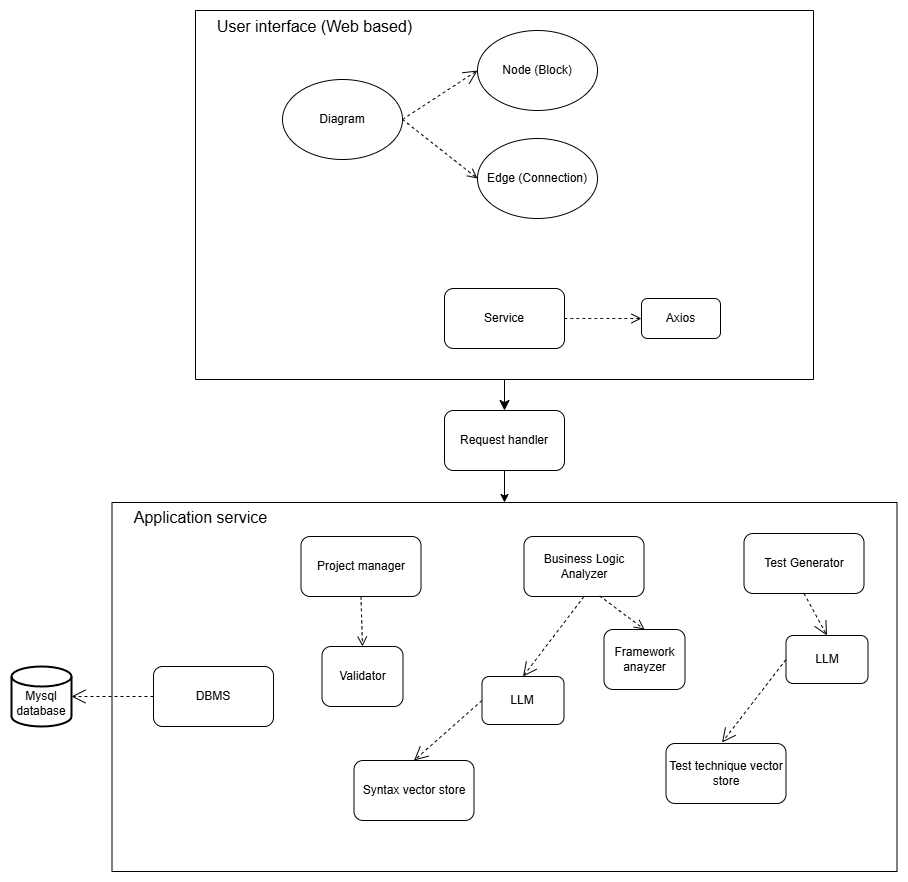
\includegraphics[width=1.0\textwidth]{images/System design.drawio.png}
	\caption{Test Genie’s overall module design}
	\label{fig:system-design}
\end{figure}



\begin{figure}[H]
	\centering
	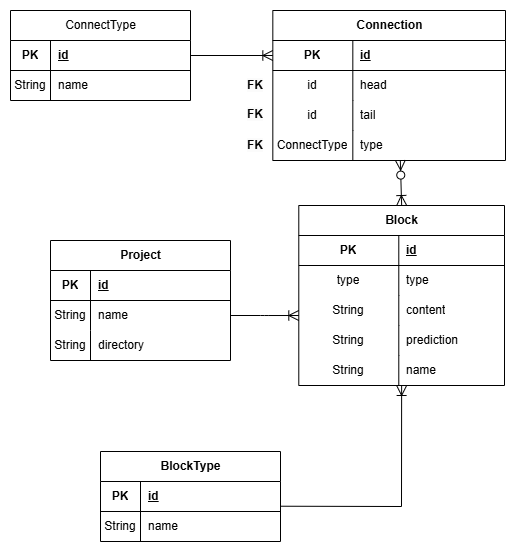
\includegraphics[width=0.8\textwidth]{images/DB block design.drawio.png}
	\caption{Block Relational Database Design}
	\label{fig:block-erd}
\end{figure}

\hspace{0.5cm}At the core of the diagram is the \textit{Block entity}, which represents distinct units of the source code identified during the project analysis. Each components stores attributes such as its type, content, prediction, and a reference to the project it belongs to. The block entity will not need to store the id of its project because it is stored as system files in the server and Backend can access it directly. This kind of design will reduce the size of the database and optimize the performance of the system.

\hspace{0.5cm} The \textit{Connection entity} defines the relationships between blocks. It uses references to two distinct blocks: head and tail, forming a directional link between them. These connections are categorized by the ConnectType entity, which stores different types of connections that can exist between blocks, such as data flow, control flow, or dependency relationships. This architecture facilitates a comprehensive understanding of the project's code structure by mapping both the functional and logical connections between different blocks.

\hspace{0.5cm}Furthermore, the \textit{BlockType entity} is used to define the classification of blocks, storing various block types such as files, classes or functions. This separation of component types allows for better categorization and analysis. The Project entity ensures that each component is tied to a specific source code directory, while ConnectType maintains clarity by classifying relationships between them. This ERD structure enables the BLA module to effectively visualize and analyze complex relationships within user projects, making it easier to identify patterns and dependencies for test generation.

\hspace{0.5cm} Just like \textit{BlockType entity}, the \textit{ConnectType entity} is used to define the classification of connections, storing various connection types such as Call, Contain, Use relationships, etc. This separation of connection types allows for better categorization and analysis. The Project entity ensures that each component is tied to a specific source code directory, while ConnectType maintains clarity by classifying relationships between them. This ERD structure enables the BLA module to effectively visualize and analyze complex relationships within user projects, making it easier to identify patterns and dependencies for test generation.
                                                                                                                                              
% connection between  each module, how they interact with each other, why each module is needed => Why this design help complete user requirement

% \begin{algorithm}[H]
% 	\small
% 	\caption{$(\text{Result}) \gets \texttt{Sample}(\text{Input1})$}
% 	\label{alg:1}
% 	\begin{algorithmic}[1]
% 		\Require $\text{Input1}$ is a predefined parameter.
% 		\State $\text{Set} \gets \emptyset$
% 		\For{$\text{element} \in \text{Input1}$}
% 		\If{$\text{Condition}(\text{element})$ is true}
% 		\State $\text{Set} \gets \text{Set} \cup \{\text{Process}(\text{element})\}$
% 		\Else
% 		\State \textbf{continue}
% 		\EndIf
% 		\EndFor
% 		\State $\text{Intermediate} \gets \texttt{Transform}(\text{Set})$
% 		\State \Return $\text{Result}$
% 	\end{algorithmic}
% \end{algorithm}

% Aenean arcu nulla, ornare sed arcu nec, mollis pharetra dolor. Maecenas rutrum efficitur dui nec rutrum. Sed suscipit, felis non malesuada ultrices, urna lorem porttitor mi, quis dignissim lectus mi a justo. Mauris erat ante, placerat eu sapien id, finibus maximus nisl. Nam cursus velit eu convallis molestie. Fusce eleifend fermentum elementum. Mauris congue non mauris a blandit. In vel ante mi. Etiam et consectetur quam, accumsan aliquam dolor. Aenean sed tristique massa.